\chapter{Segmentación, seguridad y rutas}

\section{Modelo de confianza}

La segmentación no se limita a asignar prefijos diferentes. Dentro de una VPC existe una ruta local que puede transportar paquetes entre subredes. El aislamiento efectivo surge de combinar direccionamiento, tablas de rutas, direcciones públicas y grupos de seguridad. La política adoptada es denegar por defecto y habilitar sólo flujos relacionados con la prueba o la administración.

\begin{figure}[H]
\centering
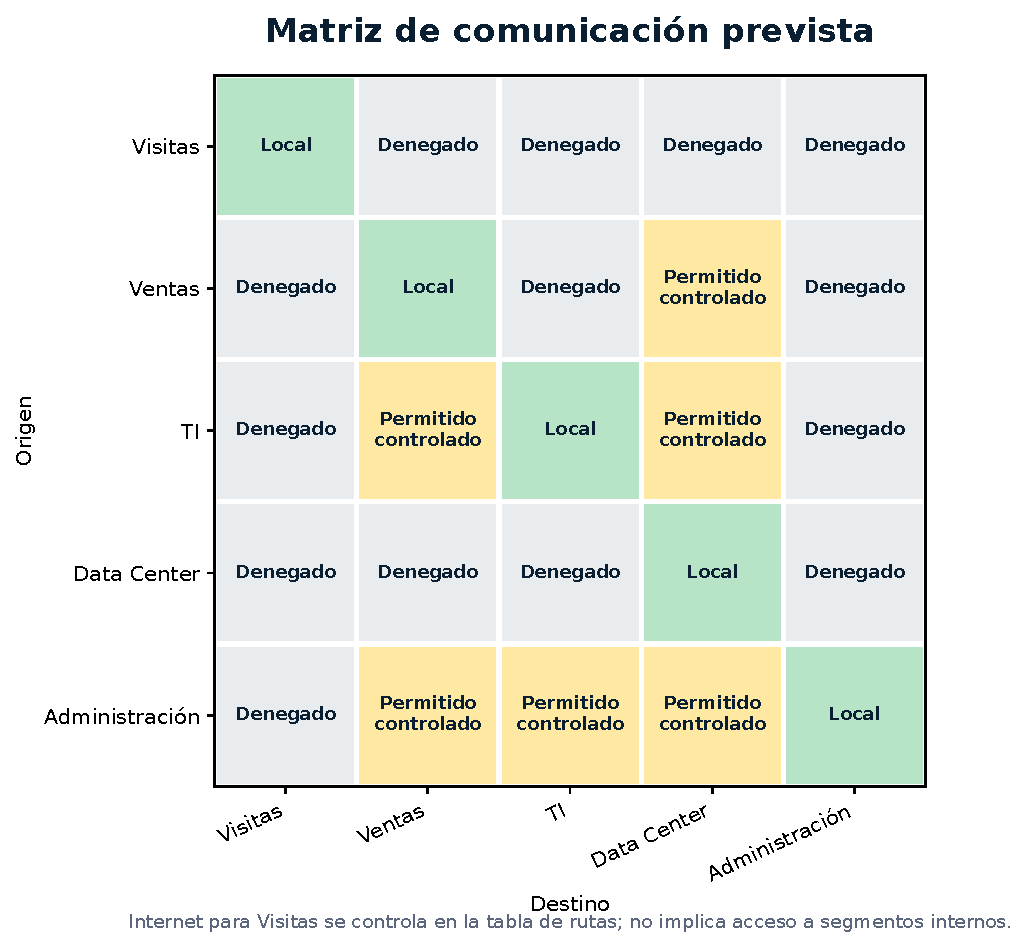
\includegraphics[width=0.83\textwidth]{matriz-seguridad.pdf}
\caption{Matriz de comunicación prevista entre segmentos. Elaboración propia.}
\label{fig:security-matrix}
\end{figure}

\section{Grupos de seguridad}

\subsection{Grupo del bastión}

La entrada TCP/22 se restringe a \code{admin\_cidr}, que debe ser una dirección IPv4 con prefijo \code{/32}. La validación de Terraform rechaza valores que no cumplan ese formato. La salida se limita al CIDR de la VPC; el bastión no necesita acceso general a Internet para ejecutar la prueba.

\subsection{Grupo de Ventas}

SSH sólo se acepta desde interfaces que pertenezcan al grupo del bastión. Esta referencia es más estable que escribir la IP privada del bastión. ICMP se acepta cuando origen y destino utilizan el mismo grupo de Ventas. La salida también se limita al \code{/24}. No existen reglas de entrada desde Visitas, Internet o un rango general.

\begin{table}[H]
\centering
\caption{Reglas relevantes del prototipo}
\begin{tabularx}{\textwidth}{p{2.7cm}p{2.0cm}p{2.2cm}Y}
\toprule
\textbf{Grupo} & \textbf{Dirección} & \textbf{Protocolo} & \textbf{Origen o destino} \\
\midrule
Bastión & Entrada & TCP/22 & IP administrativa \code{/32} \\
Bastión & Salida & Todos & \code{10.10.0.0/24} \\
Ventas & Entrada & TCP/22 & Grupo de seguridad del bastión \\
Ventas & Entrada & ICMP & El mismo grupo de seguridad \\
Ventas & Salida & Todos & \code{10.10.0.0/24} \\
\bottomrule
\end{tabularx}
\end{table}

\section{Defensa en profundidad}

Los volúmenes raíz se cifran y las instancias exigen tokens de Instance Metadata Service versión 2. No se versionan llaves privadas ni archivos de estado. El archivo \code{.gitignore} excluye \code{*.pem}, \code{*.key}, \code{terraform.tfvars}, \code{*.tfstate} y la carpeta de trabajo del proveedor.

El prototipo no agrega Network ACL personalizadas porque los grupos con estado bastan para demostrar la política y reducen el riesgo de bloquear respuestas efímeras. En producción, una ACL o firewall puede complementar el control cuando la organización necesite reglas sin estado a nivel de subred, inspección o evidencia centralizada.

\section{Amenazas operativas y controles}

\begin{longtable}{p{4.0cm}p{5.0cm}p{4.4cm}}
\toprule
\textbf{Riesgo} & \textbf{Consecuencia} & \textbf{Control} \\
\midrule
\endfirsthead
\toprule
\textbf{Riesgo} & \textbf{Consecuencia} & \textbf{Control} \\
\midrule
\endhead
SSH abierto al mundo & Intentos de acceso y exposición innecesaria. & Validación obligatoria de \code{admin\_cidr /32}. \\
Llave privada en Git & Compromiso de instancias y persistencia del secreto. & Exclusión por extensión; sólo se declara la ruta a la llave pública. \\
Instancias privadas con IP pública & Ruptura del modelo de exposición. & \code{associate\_public\_ip\_} \newline \code{address=false}. \\
Uso de metadatos sin token & Mayor exposición ante ciertas solicitudes inducidas. & IMDSv2 obligatorio. \\
Recursos olvidados & Cargos posteriores a la entrega. & Etiqueta de expiración y destrucción automatizada. \\
Permisos IAM excesivos & Daño más allá del proyecto. & Usar identidad académica separada y permisos limitados. \\
Solapamiento CIDR & Rutas ambiguas y fallas de creación. & Validación local y validación del proveedor. \\
\bottomrule
\end{longtable}

\section{Limitaciones de seguridad}

Una prueba exitosa de ping sólo confirma alcance ICMP entre dos interfaces bajo las reglas presentes. No demuestra confidencialidad del tráfico, seguridad de aplicaciones, resistencia a ataques o disponibilidad. La fase tampoco valida identidad de usuarios finales. Estas propiedades exigirían controles adicionales y pruebas específicas.
